% !TEX root = ../om_ts_09.tex

\begin{frame} % название фрагмента

\videotitle{Много сезонных составляющих}

\end{frame}



\begin{frame}{Много сезонных составляющих: план}
  \begin{itemize}[<+->]
    \item Наложение \alert{нескольких частот}.
    \item Краткое напоминание STL.
    \item MSTL = STL \alert{много раз}.
  \end{itemize}

\end{frame}

\begin{frame}
  \frametitle{Число звонков в банк}

  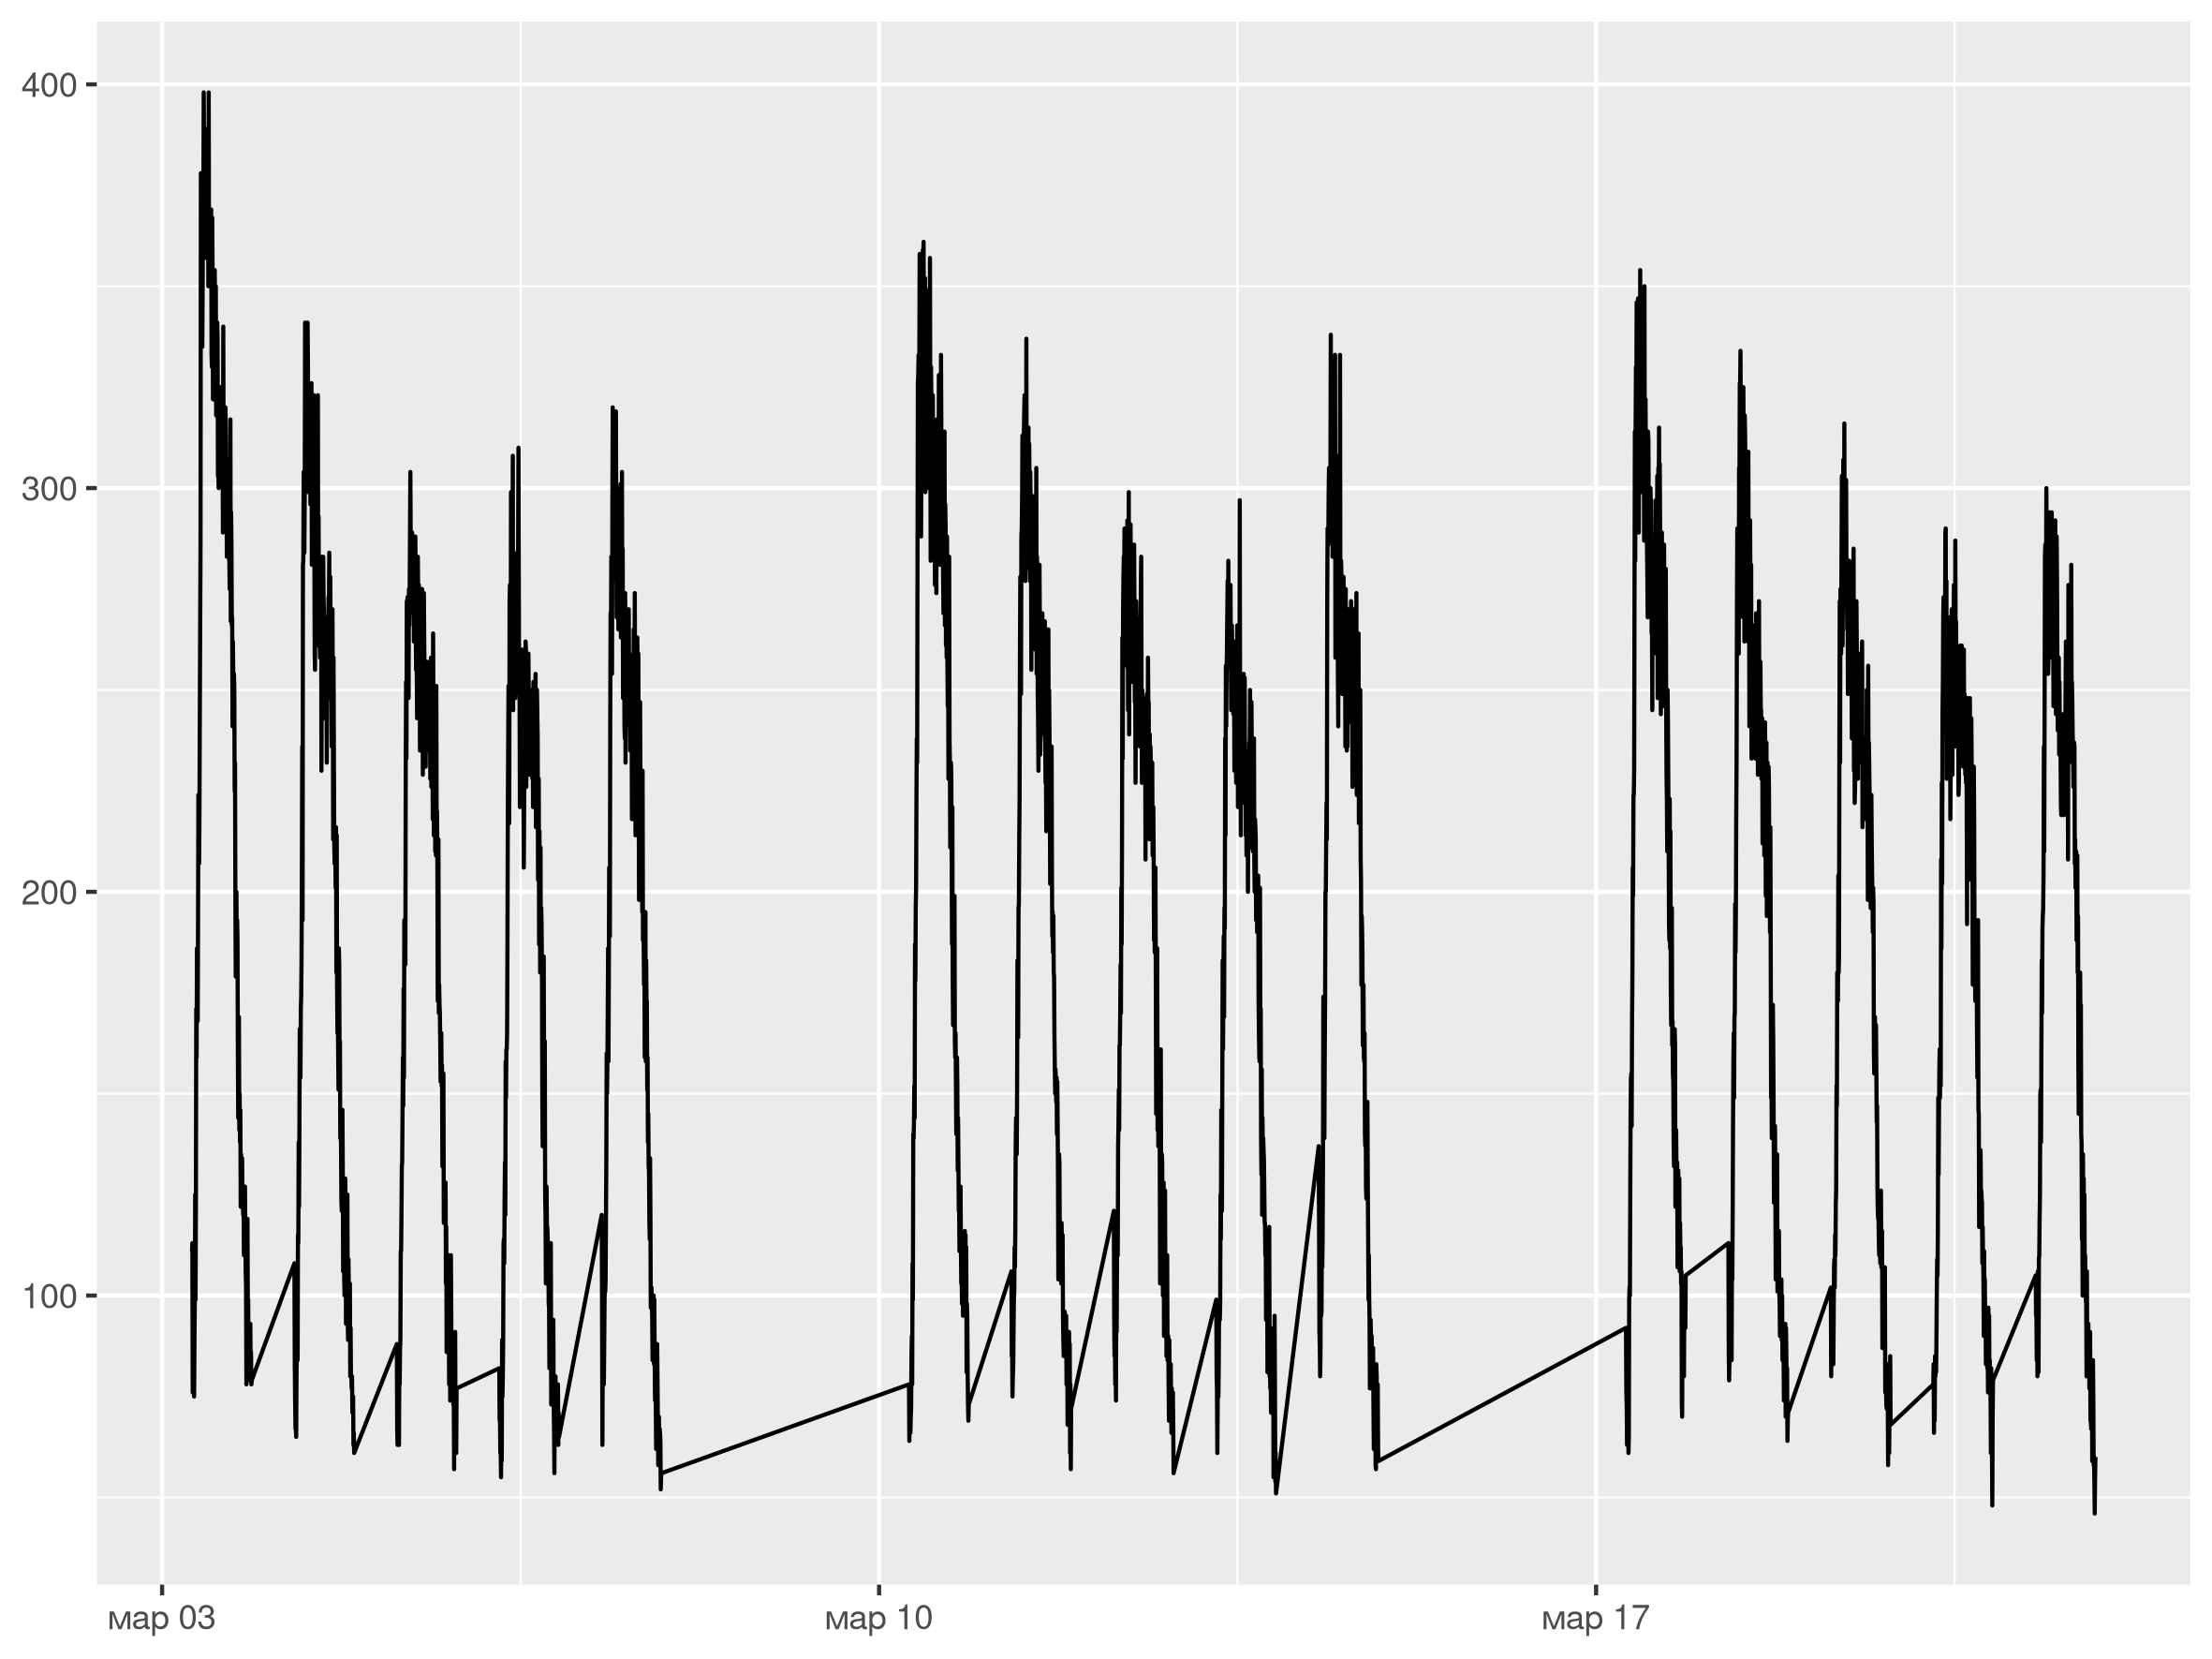
\includegraphics[width=\textwidth]{pictures/om_ts_09-006.png}

  
\end{frame}

\begin{frame}
  \frametitle{Что делать со сложной сезонностью?}

  \begin{itemize}[<+->]
    \item Использовать \alert{подходящую} модель:
    
    ARIMA + предикторы Фурье, PROPHET, TBATS, \ldots

    \item Разложить ряд на \alert{много} составляющих:
    
    \[
      y_t = trend_t + seas_t^{(1)} + seas_t^{(2)} + remainder_t
    \]
  \end{itemize}
  

\end{frame}


\begin{frame}{Вспоминаем STL}

  \alert{На входе:}
  
  Ряд $y_t$.
  \pause
  \begin{itemize}
    \item $n_p$ — периодичность сезонности, например, $n_p=12$. \pause 
    \item $n_l$ — сила сглаживания низкочастотного фильтра.   \pause
    \item $n_s$ — сила сглаживания сезонных подряд\textit{о}в. \pause
    \item $n_t$ — сила сглаживания при выделении тренда.     
  \end{itemize}

  \pause
  \alert{На выходе:}
  
  Разложение $y_t = trend_t + seas_t + remainder_t$.  
\end{frame}
  
\begin{frame}
  \frametitle{Применим STL последовательно!}

  \begin{enumerate}[<+->]
    \item \alert{Первичное} выделение сезонных компонент. 
    \item \alert{Корректировка} сезонных компонент. 
    \item Добываем тренд и остаток. 
  \end{enumerate}

\end{frame}



\begin{frame}
  \frametitle{MSTL = STL много раз!}

  Шаг 1. Первичное выделение сезонных компонент. 

  \begin{enumerate}[<+->]
    \item Запустим STL для выделения сезонности \alert{высокой частоты}. 
    
    Запомним выделенную компоненту $seas_t^{(1)}$ и удалим её из ряда, $y_t^{(-1)} = y_t - seas_t^{(1)}$. 

    \item Запустим STL для выделения сезонности \alert{средней частоты}. 
    
    Запомним выделенную компоненту $seas_t^{(2)}$ и удалим её из ряда, $y_t^{(-1,2)}= y_t^{(-1)} - seas_t^{(2)}$. 

    \item \ldots

  \end{enumerate}

\end{frame}



\begin{frame}
  \frametitle{Уточняем сезонные компоненты}

  Шаг 2. Корректировка сезонных компонент. 

  \begin{enumerate}[<+->]
    \item Временно \alert{возвращаем} в полностью очищенный ряд найденную \alert{сезонность} высокой частоты.
    
    Запускаем STL и получаем \alert{уточнённую компоненту} $seas_t^{(1)}$, удаляем её из ряда и получаем \alert{уточнённый очищенный ряд}. 

    \item Временно \alert{возвращаем} в полностью очищенный ряд найденную \alert{сезонность} средней частоты.
    
    Запускаем STL и получаем \alert{уточнённую компоненту} $seas_t^{(2)}$, удаляем её из ряда и получаем \alert{уточнённый очищенный ряд}. 

    \item \ldots

  \end{enumerate}

\end{frame}



\begin{frame}
  \frametitle{Завершаем алгоритм}

  Шаг 3. Добываем тренд и остаток. 

  \alert{Тренд} и \alert{остаток} берем из самого \alert{последнего} STL разложения, уточнявшего сезонные компоненты. 
  
\end{frame}


\begin{frame}{Много сезонных составляющих: итоги}

  \begin{itemize}[<+->]
    \item \alert{MSTL} — быстрый и устойчивый алгоритм разложения ряда.
    \item Теоретически \alert{MSTL} может работать с пропусками.
    \item Есть другие алгоритмы: ARIMA + предикторы Фурье, TBATS, PROPHET, \ldots
  \end{itemize}
\end{frame}

